\section{Walking task}
% presentation de la dynamique et hypothèse

\setcounter{subsection}{1}
\begin{frame}{Walking pattern generator}

  \begin{center}
    \scalebox{1.0}{%!TEX root = ../../14-icra-RealTimeNMPC.tex

\tikzstyle{block} = [draw, fill=blue!20, rectangle,
    minimum height=2em, minimum width=5em, align=center]
\tikzstyle{sum} = [draw, fill=blue, circle, node distance=1cm]
\tikzstyle{input} = [coordinate]
\tikzstyle{output} = [coordinate]
\tikzstyle{pinstyle} = [pin edge={to-,thin,black}]

% The block diagram code is probably more verbose than necessary
\begin{tikzpicture}[auto, node distance=2cm,>=latex]
\normalsize
    % We start by placing the blocks
    \node [input]  at (-2, 0.0) (input)  {};
    \node [sum]    at ( -0.5, 0.0) (sumin)  {};
    \node [sum]    at ( 7.5, 0.0) (sumout) {};
    \node [output] at ( 8.5, 0.0) (output) {};

    % SQP Controller Block
    \node [block] at (3.5,0) (controller) {
        \normalsize real time SQP Controller \\
        \normalsize Orientation $+$ Position
    };
    % System Block
    \node [block] at (3.5, -2) (system) {
            \normalsize Generalized Inverse Kinematics\\
             \normalsize Robot
        };
    
    % PATHS
    \draw [draw,->] (input) -- node {$
        \mathbf{v}^{\mathrm{ref}}
    $} (sumin);
    \draw [->] (controller) -- node[name=u, align=center] {
    $\begin{matrix}
        \hat{c}_{k+1}^{x,y,\theta}\\
        \hat{f}_{k+1}^{x,y,\theta}
    \end{matrix}$
    } (sumout);
    \draw [draw,->] (sumout) -- node {$
    $} (output);
    \draw [->] (sumin) -- node {} (controller);
    \draw [->] (sumout) |- node[near start] {}   (system);
    \draw [- ] (sumout) |- node {} (-0.5, -1.0);
    \draw [->] (-0.5, -1.0) -- node {} (sumin);

\end{tikzpicture}
} \\
  \end{center}

  \textbf{\color{blue}HRP-2 under actuation control compute : }
    \begin{enumerate}
    \item the CoM trajectory w.r.t. a
        reference velocity ($\mathbf{v}^{\mathrm{ref}} = [v_x,\;v_y,\;v_\theta] $)
    \item the feet positions and orientations
    \end{enumerate}
  \textbf{\color{blue}Nice feature embedded (obstacle avoidance, reactive walking, ...)}\\
  \textbf{\color{blue}Cost $2ms$ in computation times on dual core $2.8GHz$}
\end{frame}


\begin{frame}{Walking pattern generator}
  \begin{center}
    \hspace*{-0.5cm}
    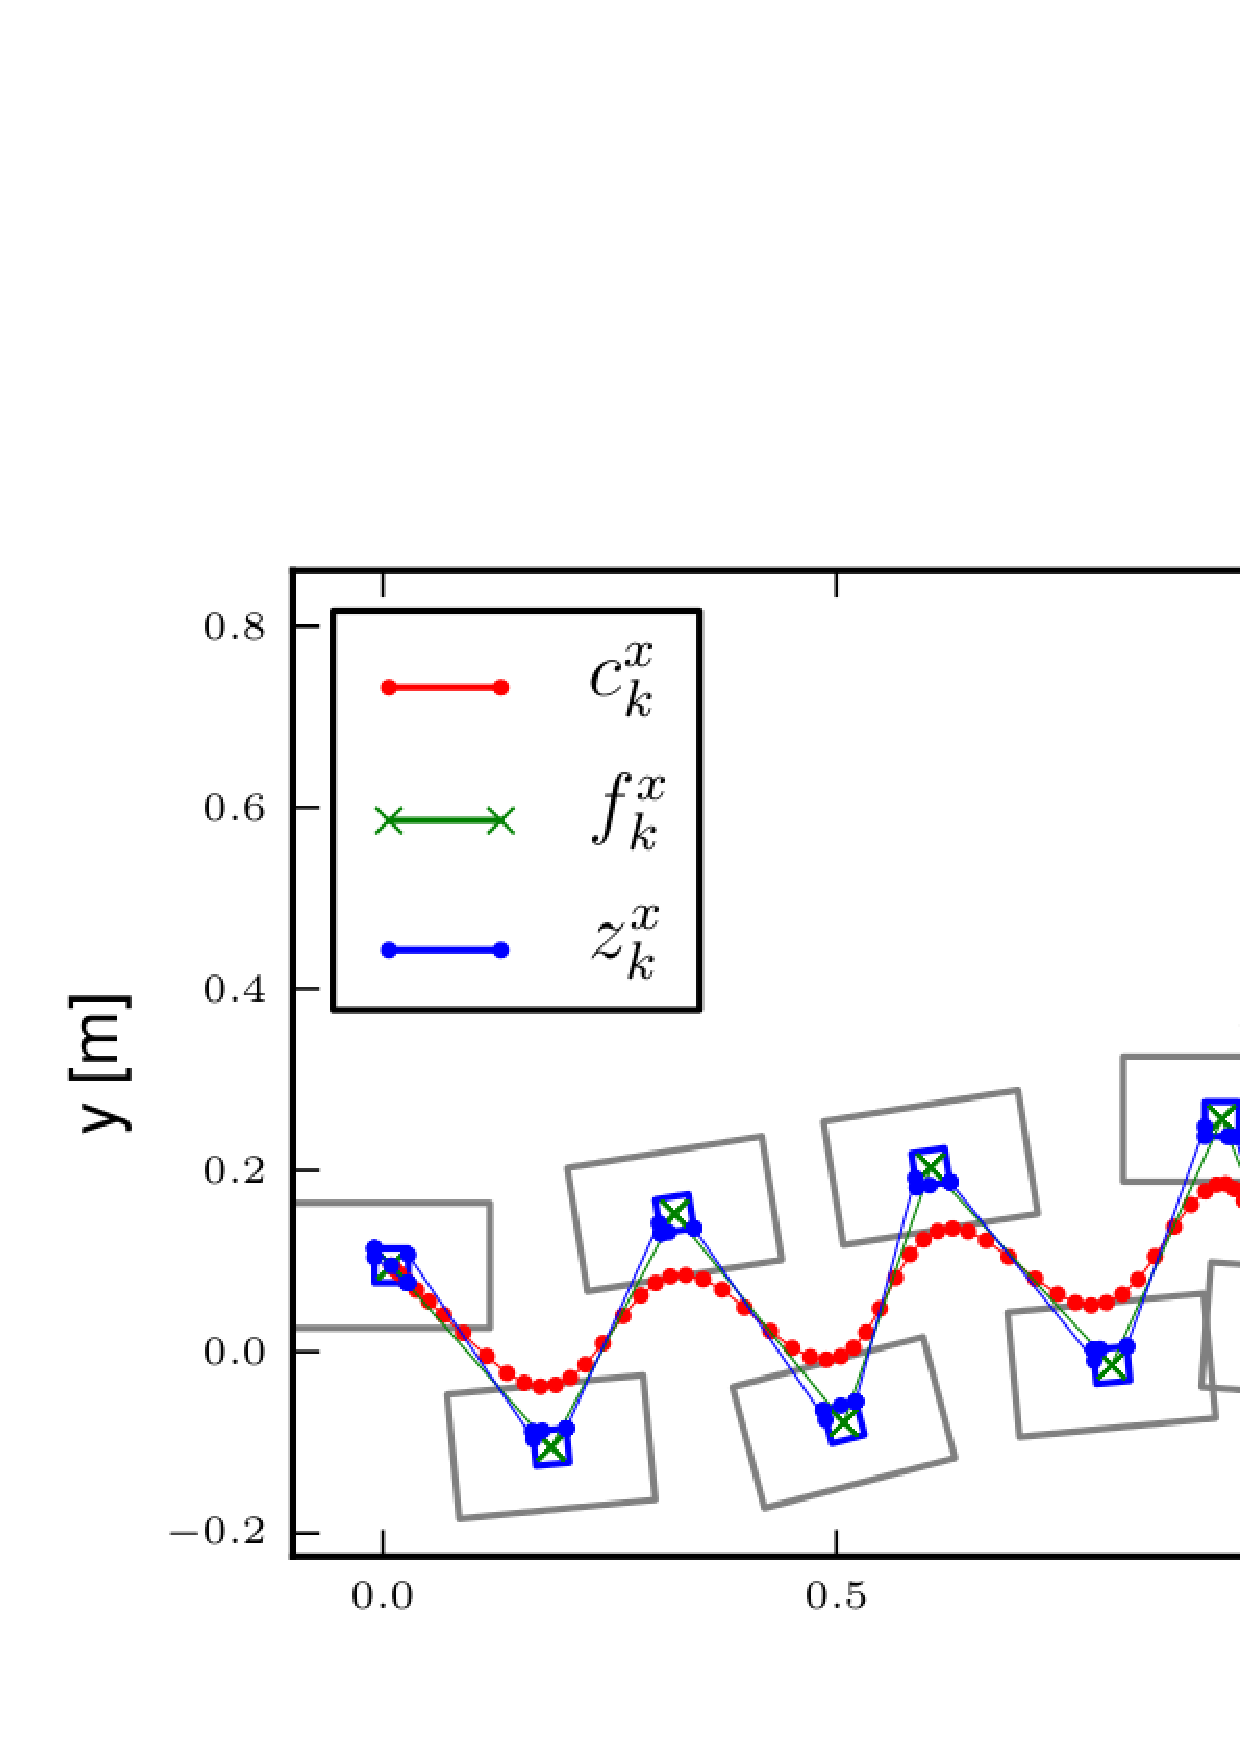
\includegraphics[height=5cm]{nmpc_vs_classic_nmpc_motion.pdf}\\
    \textbf{\color{blue} Example of output}
  \end{center}
  \fullcite{naveau:ral:2016}
\end{frame}

\begin{frame}{Walking task}
  \vspace*{0.5cm}
  \tikzstyle{na} = [baseline=-.5ex]
  \begin{itemize}
    \item adaptive gains
      \tikz[na] \node[coordinate] (l) {};
    \item referenced velocity 
      \tikz[na] \node[coordinate] (vr) {};
  \end{itemize}
%
  \vspace*{-0.5cm}
  \begin{align*}
    \tikz[baseline]{
      \node[fill=red!40,anchor=base] (v)
      { $ \mathbf{v}^{\mathrm{ref}} $ };
    }
    = - \tikz[baseline]{
      \node[fill=purple!40,anchor=base] (l1)
      {$\lambda$};
    } \;
    \tikz[baseline]{
      \node[fill=blue!20,anchor=base] (e1)
      {$ \mathbf{e}_{w} $};
    } - 
    \tikz[baseline]{
      \node[fill=purple!40,anchor=base] (l2)
      {$ \mathbf{\Lambda} $};
    }
    \int \tikz[baseline]{
      \node[fill=blue!20,anchor=base] (e2)
      {$ \mathbf{e}_{w} $};
    } dt
  \end{align*}
  \vspace*{-0.5cm}
  \begin{itemize}
    \item $ \mathbf{e}_{w} = \mathbf{x} - \mathbf{x}_{d} $
    \tikz[na] \node[coordinate] (e) {}; \\[0.2cm]
    $\mathbf{x} = [ x_{chest} \; y_{chest} \; \theta_{chest} ]$
  \end{itemize}
%
% Now it's time to draw some edges between the global nodes. Note that we
% have to apply the 'overlay' style.
  \begin{tikzpicture}[overlay]
    \path[->,line width=0.5mm, red!100!black!80]<2-> (vr) edge [bend left] (v);
    \path[->,line width=0.5mm, blue!50!black!70]<3-> (e) edge [bend right] (e1);
    \path[->,line width=0.5mm, blue!50!black!70]<3-> (e) edge [bend right] (e2);
    \path[->,line width=0.5mm, purple!100!black!80]<4-> (l) edge [bend left] (l1);
    \path[->,line width=0.5mm, purple!100!black!80]<4-> (l) edge [bend left] (l2);
  \end{tikzpicture}
%  
\end{frame}


\begin{frame}{Localization of the chest}
  \vspace*{0.5cm}
  \begin{center}
    \includegraphics[angle=90, height=0.35\paperheight]{./DSC00610.JPG}
    \hspace*{1.5cm}
    \includegraphics[height=0.35\paperheight]{./camera_raptor.jpeg}
  \end{center}
   \textbf{\color{blue} The robot position is measure via a motion capture system}\\
\end{frame}
